\begin{enumerate}[label=\thesubsection.\arabic*.,ref=\thesubsection.\theenumi]
\numberwithin{equation}{enumi}
\item Plot the polar plot of 
\begin{align}
G(s) = \frac{1}{(s+1)(s+2)(s+3)}. 
\end{align}

\solution


\begin{figure}[!ht]
\centering
  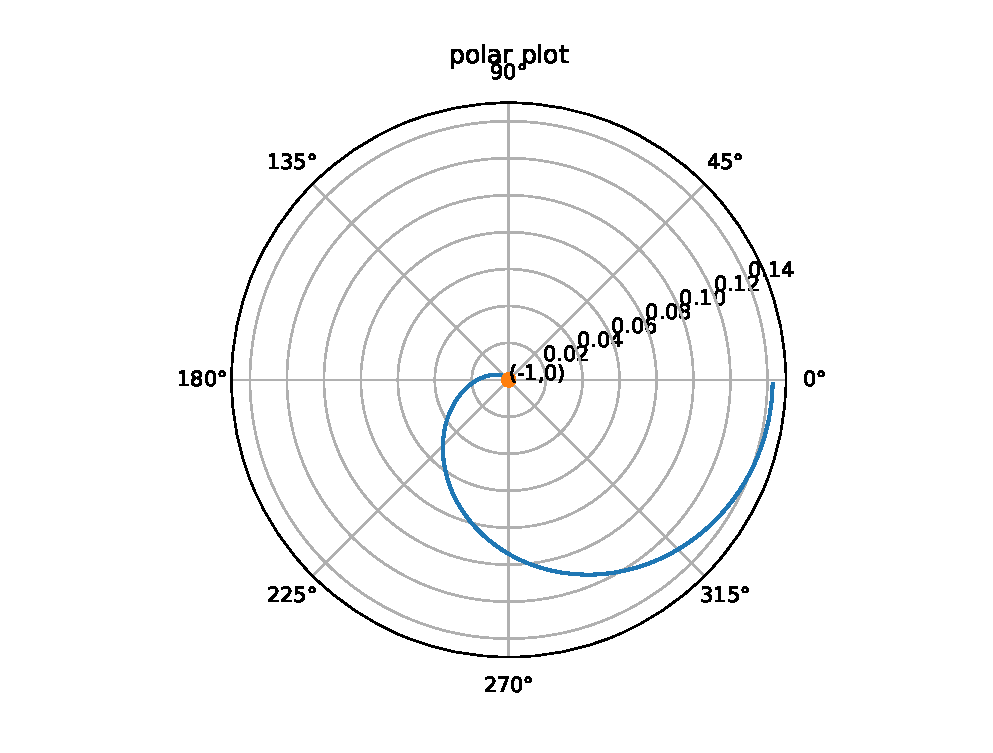
\includegraphics[width=\columnwidth]{./figs/ee18btech11033.eps}
\caption{}
  \label{fig:ee18btech11033}
  \label{fig:ee18btech11033}
\end{figure}

The following python code generates the polar plot in Fig.   \ref{fig:ee18btech11033}

\begin{lstlisting}
codes/ee18btech11033.py
\end{lstlisting}
$\because$  (-1,0) is on the right side of the polar plot, the system is unstable.

\end{enumerate}
